\documentclass[11pt]{article}
\usepackage{amsmath, amssymb, amsthm}
\usepackage[margin=1in]{geometry}
\usepackage{setspace}
\usepackage{booktabs}
\usepackage{graphicx}
\usepackage{placeins}
\graphicspath{{figures/}}
\setstretch{1.15}

\newtheorem{theorem}{Theorem}[section]
\newtheorem{proposition}[theorem]{Proposition}
\newtheorem{corollary}[theorem]{Corollary}
\newtheorem{lemma}[theorem]{Lemma}
\newtheorem{definition}[theorem]{Definition}
\newtheorem{assumption}{Assumption}

\title{Trade Tariffs and Exchange Rates in a Multilateral World\\ \large Theoretical derivations}
\author{Jason Lu \and Dimitre Milkov}
\date{\today}

\begin{document}
\maketitle

\section{Introduction}

In a two-country model, an import tariff appreciates the tariffing country's currency under the Marshall--Lerner condition. With more than two countries, a tariff on one trading partner also reallocates expenditure across foreign suppliers, so bilateral exchange rates need not all move in the same direction.

These notes characterize the exchange-rate effects of tariffs in an $N$-country model. The general log-linearized equilibrium response is $(-J)^{-1}F$, where $F$ gives the trade-balance effects of a tariff at unchanged exchange rates and $J$ is the Jacobian of trade balances with respect to exchange rates. Under a multilateral Marshall--Lerner (MML) condition on $J$, this representation separates the trade-balance effects of the tariff from the exchange-rate adjustment required to restore equilibrium.

Under partner symmetry, the response to any tariff vector further separates into an average-protection component and a relative-treatment component; Section~\ref{sec:general} derives this decomposition without imposing the nested-CES model. Average protection determines the tariffing country's nominal effective exchange rate (NEER), while relative treatment determines the dispersion of bilateral exchange-rate responses around it. Section~\ref{sec:model} then gives the two response coefficients economic content in a nested-CES model, showing how they depend on substitution elasticities, expenditure shares, and the number of countries. For a unilateral tariff, the tariffing country always appreciates against the targeted partner and its NEER always appreciates, but its exchange rate against an untariffed bystander can move in either direction. A bystander depreciation of the tariffing country's currency occurs only when substitution across foreign import origins is sufficiently strong relative to the other trade-balance effects of the tariff (Section~\ref{sec:unilateral}). Proofs are collected in Appendix~\ref{app:proofs}.

\section{Tariffs and Exchange-Rate Adjustment}

\label{sec:general}

The results in this section require only that trade balances are differentiable with respect to exchange rates and tariffs, and do not depend on our specific nested-CES model structure.

\subsection{The bilateral case}

\label{sec:bilateral}

Consider first two countries, $A$ and $B$. Let $e_{AB}$ be units of $A$'s currency per unit of $B$'s, so that a rise in $e_{AB}$ is a depreciation of $A$, and write $\nu\equiv d\log e_{AB}$. Let $A$'s trade balance $\mathrm{TB}_A$ be a differentiable function of $\nu$ and of a tariff $\tau$ that $A$ levies on $B$. Linearizing at a balanced free-trade baseline,
\begin{equation}
d\,\mathrm{TB}_A=\mathrm{TB}_{A\nu}\,\nu+\mathrm{TB}_{A\tau}\,d\tau,
\qquad
\mathrm{TB}_{A\nu}\equiv\frac{\partial\,d\mathrm{TB}_A}{\partial\nu},
\qquad
\mathrm{TB}_{A\tau}\equiv\frac{\partial\,d\mathrm{TB}_A}{\partial\tau}\bigg|_{\nu\ \mathrm{fixed}} .
\label{eq:bilat}
\end{equation}
The tariff raises the domestic price of imports and so improves $A$'s trade balance at unchanged exchange rates, $\mathrm{TB}_{A\tau}>0$. Restoring balance then requires
\begin{equation}
\nu^{\ast}=-\frac{\mathrm{TB}_{A\tau}}{\mathrm{TB}_{A\nu}}\,d\tau ,
\label{eq:bilat-slope}
\end{equation}
which is an appreciation if and only if $\mathrm{TB}_{A\nu}>0$, that is, if and only if a depreciation improves $A$'s trade balance. This is the ordinary Marshall--Lerner condition; Section~\ref{sec:twocountry} shows that in the nested-CES model it takes the familiar elasticity form $\varepsilon_X+\varepsilon_M>1$.

The two steps in \eqref{eq:bilat}--\eqref{eq:bilat-slope} are the whole of the adjustment logic: the tariff first displaces the trade balance at unchanged exchange rates, and the exchange rate then moves to absorb that displacement. Figure~\ref{fig:twocountry} displays them.

\begin{figure}[htbp]
\centering
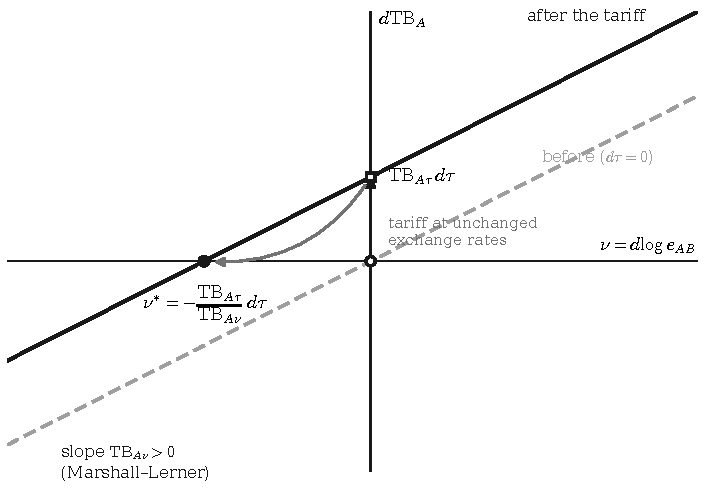
\includegraphics[width=0.72\textwidth]{fig1_two_country.pdf}
\caption{Bilateral equilibrium adjustment. The schedule is \eqref{eq:bilat}; its slope $\mathrm{TB}_{A\nu}$ is positive exactly under the Marshall--Lerner condition. At unchanged exchange rates the tariff shifts the schedule up by $\mathrm{TB}_{A\tau}\,d\tau>0$ (open square). The currency then appreciates along the new schedule until balance is restored at $\nu^{\ast}=-(\mathrm{TB}_{A\tau}/\mathrm{TB}_{A\nu})\,d\tau$.}
\label{fig:twocountry}
\end{figure}

\subsection{The local disturbance--adjustment representation}

\label{sec:representation}

Consider any differentiable multilateral trade environment with $N-1$ independent trade-balance conditions, $\mathrm{TB}_i = 0$ for $i \neq A$, which are each functions of exchange rates and tariffs. Stack the exchange-rate changes as $\nu \equiv (\nu_j)_{j \neq A}$, $\nu_j\equiv d\log e_{Aj}$, and the bilateral tariff changes as $d\boldsymbol\tau \equiv (dt_{jk})_{j \neq k}$, so that $\nu$ and $d\boldsymbol\tau$ are the perturbation vectors of the levels $e_{Aj}$ and $\tau_{jk}$. The conditions for $i \neq A$ are
\begin{equation}
J\, \nu + G\, d\boldsymbol\tau = 0,
\qquad
J_{il} \equiv \frac{\partial\, d\mathrm{TB}_i}{\partial \nu_l},
\qquad
G_{i,(jk)} \equiv \frac{\partial\, d\mathrm{TB}_i}{\partial t_{jk}}\bigg|_{\nu \text{ fixed}} .
\label{eq:JFdef}
\end{equation}
A tariff experiment fixes a \emph{pattern} of tariff changes $a$ and a scalar \emph{magnitude} $d\tau$, so that $d\boldsymbol\tau = a\,d\tau$. Defining
\begin{equation}
F \equiv G\,a ,
\label{eq:Fdef}
\end{equation}
the vector of fixed-exchange-rate trade-balance disturbances generated by one unit of that pattern, the equilibrium conditions become
\begin{equation}
J\, \nu = -F\, d\tau,
\qquad
\nu = (-J)^{-1} F\, d\tau .
\label{eq:system}
\end{equation}
Thus $F$, and more generally $G$, gives the trade-balance effects of the tariff at unchanged exchange rates, including substitution and income effects; $J$ describes how trade balances respond to exchange-rate changes; and $(-J)^{-1}$ maps the disturbance into the equilibrium exchange-rate changes that absorb it.

At $N=2$ there is a single condition, $\mathrm{TB}_B=0$. Since $d\,\mathrm{TB}_B=-d\,\mathrm{TB}_A$, the scalars in \eqref{eq:JFdef} are $-J=\mathrm{TB}_{A\nu}$ and $F=-\mathrm{TB}_{A\tau}$, and \eqref{eq:system} is exactly \eqref{eq:bilat-slope}. The $N$-country system is the matrix analogue of that scalar problem.

\subsection{The multilateral Marshall--Lerner condition}

\label{sec:mml}

At $N=2$, the requirement that exchange-rate adjustment stabilizes the trade balance is the scalar condition $-J = \mathrm{TB}_{A\nu} > 0$ of Section~\ref{sec:bilateral}. The $N$-country generalization requires that the adjustment mapping $(-J)^{-1}$ be well defined and positive.

\begin{definition}[Multilateral Marshall--Lerner condition]
The adjustment mechanism satisfies the \emph{multilateral Marshall--Lerner condition} (MML) if
\begin{equation}
-J \ \text{is a nonsingular M-matrix:}
\qquad
J_{il} \geq 0 \ \ (l \neq i)
\quad
\text{and}
\quad
(-J)^{-1} \ \text{exists with} \ (-J)^{-1} \geq 0 .
\label{eq:invpos}
\end{equation}
\label{def:mml}
\end{definition}

\noindent By \eqref{eq:system}, under MML, each exchange-rate response is a nonnegative-weighted combination of the trade-balance effects at fixed exchange rates. Writing $\vartheta_{ij}\equiv\big[(-J)^{-1}\big]_{ij}\geq0$,
\begin{equation}
\frac{d\nu_i}{d\tau}=\sum_j\vartheta_{ij}F_j ,
\label{eq:signrule}
\end{equation}
so $\vartheta_{ij}$ measures the response of currency $i$ to a unit trade-balance disturbance in country $j$. A uniformly signed $F$ therefore cannot generate exchange-rate responses of the opposite sign. When $F$ has mixed signs, the response of any individual exchange rate depends on the full vector of trade-balance effects rather than on the corresponding element $F_i$ alone. The condition also implies $\det(-J) > 0$, which is used in the threshold calculations below. At $N = 2$, the system is scalar and the condition reduces to $\mathrm{TB}_{A\nu}>0$, the ordinary Marshall--Lerner condition.

The condition above is stated directly on $J$, but it can alternatively be obtained from a restriction on the full bilateral Jacobian. Let $\widetilde J$ be the full $N \times N$ Jacobian, so that $J$ is $\widetilde J$ with row and column $A$ deleted. Two identities hold for $\widetilde J$. Each trade balance is homogeneous of degree one in currency values, so by Euler's theorem row $i$ sums to $\mathrm{TB}_i$, which is zero at a balanced baseline; and Walras' law, $\sum_i \mathrm{TB}_i \equiv 0$, ensures that the columns sum to zero. Thus
\begin{equation}
\sum_l \widetilde J_{il} = 0
\quad
\forall i,
\qquad
\qquad
\sum_i \widetilde J_{il} = 0
\quad
\forall l .
\label{eq:hom}
\end{equation}
The row identity pins down each diagonal entry of $\widetilde J$ from its off-diagonal entries, so a sign restriction on the off-diagonal entries alone determines the own effects and, after deleting $A$, the dominance of $J$. This gives a sufficient condition for MML.

\begin{assumption}[Gross substitutability]
$\widetilde J_{il} \geq 0$ for all $l \neq i$.
\label{as:gs}
\end{assumption}

An appreciation of currency $l$ raises the price of $l$'s goods, and Assumption~\ref{as:gs} says that this improves every other country's trade balance: tradables are gross substitutes across countries. With the row identity in \eqref{eq:hom}, $\widetilde J_{ii} = -\sum_{l \neq i}\widetilde J_{il} \leq 0$, and deleting row and column $A$ gives
\begin{equation}
|J_{ii}| - \sum_{l \neq i,\,A} J_{il} = \widetilde J_{iA} \;\geq\; 0 ,
\label{eq:diagdom}
\end{equation}
so $J$ is diagonally dominant, strictly in every row with $\widetilde J_{iA} > 0$.

\begin{lemma}[Sufficiency of gross substitutability]
Under Assumption~\ref{as:gs}, with $J$ irreducible and $\widetilde J_{iA} > 0$ for some $i$, MML \eqref{eq:invpos} holds.
\label{res:mml}
\end{lemma}

\noindent The proof is in Appendix~\ref{app:proofs}.

\subsection{Symmetric partners}

\label{sec:exch}

Restrict attention to tariffs imposed by $A$, and write $t = (t_j)_{j \neq A}$ with $t_j \equiv dt_{Aj}$ for $A$'s own tariff vector, so that $G$ in \eqref{eq:JFdef} is $(N-1) \times (N-1)$. Suppose that $A$'s trading partners are symmetric: relabeling them leaves the reduced system unchanged, $PJP' = J$ and $PGP' = G$ for every permutation matrix $P$ of the $N-1$ partners. This holds when the partners have identical sizes, trade weights, and parameters at the baseline; $A$ itself need not be symmetric with them. Take $N \geq 3$.

Under partner symmetry, the tariff vector can affect exchange rates through only two components: average protection, the average tariff across partners, and relative treatment, the differences in tariffs across partners. Decompose
\begin{equation}
t = \bar t\,\mathbf{1} + \tilde t,
\qquad
\bar t \equiv \frac{1}{N-1}\mathbf{1}'t,
\qquad
\mathbf{1}'\tilde t = 0 .
\label{eq:t-split}
\end{equation}
Componentwise this is
\begin{equation}
t_j = \bar t + (t_j - \bar t),
\qquad
\tilde t_j \equiv t_j - \bar t .
\label{eq:t-split-scalar}
\end{equation}
We refer to $\bar t\,\mathbf{1}$ as \emph{average protection} and to $\tilde t$ as \emph{relative treatment}: average protection is the tariff level $A$ applies to its partners on average, and relative treatment records how each partner is taxed relative to that average. Mathematically, $\mathbf{1}$ spans the \emph{scale} eigenspace of constant vectors and $\tilde t$ lies in the \emph{discriminatory} eigenspace of zero-sum vectors; we use the latter terms only where the eigenspace structure itself is at issue.

Let $d\nu_A^E\equiv\frac{1}{N-1}\sum_{j\neq A}\nu_j$ denote the equally weighted average of $A$'s bilateral responses, which under symmetry is $A$'s nominal effective exchange rate \eqref{eq:neer}.

\begin{proposition}[Average protection and relative treatment]
Suppose $A$'s partners are symmetric and $N\geq3$. Then $-J$ and $G$ each have exactly two eigenvalues, one on $\operatorname{span}\{\mathbf 1\}$ and one on $\{v:\mathbf 1'v=0\}$; write these $j_S,j_D$ and $g_S,g_D$ respectively. If $j_S,j_D\neq0$, the response to any tariff vector $t$ imposed by $A$ is
\begin{equation}
\nu = \lambda_S\,\bar t\,\mathbf{1} + \lambda_D\,\tilde t ,
\qquad
\lambda_S \equiv \frac{g_S}{j_S},
\qquad
\lambda_D \equiv \frac{g_D}{j_D} ,
\label{eq:decomp}
\end{equation}
so that average protection alone determines the effective exchange rate and relative treatment alone determines the dispersion of bilateral rates around it and the cross rates among partners:
\begin{equation}
d\nu_A^E = \lambda_S\,\bar t ,
\qquad
\nu_j - d\nu_A^E = \lambda_D\,\tilde t_j ,
\qquad
d\log e_{jk} = \lambda_D\,(t_k-t_j) .
\label{eq:decomp-parts}
\end{equation}
MML \eqref{eq:invpos} holds if and only if
\begin{equation}
j_S > 0
\qquad
\text{and}
\qquad
j_D \geq j_S .
\label{eq:mml-eigen}
\end{equation}
\label{res:decomp}
\end{proposition}

\noindent The reason the response takes this two-term form is that any matrix invariant to relabeling the partners has the form $aI + b\,\mathbf{1}\mathbf{1}'$. With $\mathbf{1}'\mathbf{1} = N-1$ and $\mathbf{1}'\tilde t = 0$,
\begin{equation*}
(aI + b\,\mathbf{1}\mathbf{1}')\,t = \big(a + (N-1)b\big)\,\bar t\,\mathbf{1} + a\,\tilde t .
\end{equation*}
The matrix therefore acts separately on average protection and relative treatment, with eigenvalues $a+(N-1)b$ on $\operatorname{span}\{\mathbf 1\}$ and $a$ on the zero-sum subspace. For $-J$ and $G$ these are
\begin{equation}
\begin{aligned}
-J &= a_J I + b_J\,\mathbf{1}\mathbf{1}' : & j_S &= a_J + (N-1)\,b_J, & j_D &= a_J ,\\
G  &= a_G I + b_G\,\mathbf{1}\mathbf{1}' : & g_S &= a_G + (N-1)\,b_G, & g_D &= a_G .
\end{aligned}
\label{eq:jg-eigen}
\end{equation}
Since relative treatment sums to zero, it also has no effect on the equally weighted average of the bilateral exchange rates, which is the first equality in \eqref{eq:decomp-parts}.

Proposition~\ref{res:decomp} is model-free: it says only that exchangeability reduces the adjustment problem to two scalars, without saying what those scalars are. Section~\ref{sec:symmetric} computes them for the nested-CES model.

\section{The Nested-CES Model}

\label{sec:model}
\label{sec:symmetric}

We now specify the $N$-country model whose matrices $J$ and $G$ the rest of the paper characterizes, and specialize the general results of Section~\ref{sec:general} to it.

\subsection{Production, preferences, and equilibrium}

\label{sec:setup}

Countries are indexed by $i,j \in \{1,\dots,N\}$. Where useful, we use $A$ for the tariffing country, $B$ for the tariff target, and $C$ for an untariffed bystander. Each country produces a country-specific tradable and a non-tradable from labor:
\begin{equation*}
Y_{T_i}=A_{T_i}L_{T_i}, \qquad Y_{N_i}=A_{N_i}L_{N_i}, \qquad L_{T_i}+L_{N_i}=L_i,
\end{equation*}
with perfect competition and the producer-price normalization $P_{T_i}=1$ in $i$'s currency, so
\begin{equation*}
w_i=A_{T_i}, \qquad P_{N_i}=A_{T_i}/A_{N_i}.
\end{equation*}
Wages are constant in own currency, so relative adjustment occurs through exchange rates.

Preferences are nested CES:
\begin{align*}
C_i &= C_{T_i}^{\alpha_T}C_{N_i}^{1-\alpha_T}
&& \text{(tradable share } \alpha_T),\\[2pt]
C_{T_i} &= \Big[\alpha_D^{1/\eta}C_{T_i i}^{\frac{\eta-1}{\eta}}
+(1-\alpha_D)^{1/\eta}M_i^{\frac{\eta-1}{\eta}}\Big]^{\frac{\eta}{\eta-1}}
&& \text{(home weight } \alpha_D,\text{ elasticity } \eta),\\[2pt]
M_i &= \Big[\textstyle\sum_{j\neq i}\beta_{ij}^{1/\rho}C_{T_j i}^{\frac{\rho-1}{\rho}}\Big]^{\frac{\rho}{\rho-1}}
&& \text{(origin weights } \beta_{ij},\text{ elasticity } \rho).
\end{align*}
The nesting is chosen precisely to separate the two substitution margins that the adjustment problem turns on: the elasticity $\eta$ governs substitution between domestic and imported tradables, while $\rho$ governs substitution across foreign origins conditional on importing. The latter margin is inactive at $N=2$ and active at $N\geq3$.

The \emph{symmetric benchmark} imposes $\beta_{ij}=1/(N-1)$, common parameters $(\alpha_T,\alpha_D,\eta,\rho)$, and equal endowments and productivities. Home bias remains through $\alpha_D$. Full symmetry between domestic and foreign tradables would additionally require $\rho=\eta$ and $\alpha_D=1/N$, which we do not impose.

Define $e_{ij}$ as units of $i$'s currency per unit of $j$'s, with $e_{ii}=1$ and $e_{ij}=e_{ik}e_{kj}$. A rise in $e_{ij}$ is therefore a depreciation of $i$ against $j$. Log changes in bilateral exchange rates relative to $A$ are denoted by $\nu_j\equiv d\log e_{Aj}$, with $\nu_A=0$.

Tariffs $\tau_{ij}\geq0$ are ad valorem and are levied by $i$ on imports from $j$, with $\tau_{ii}=0$. Consumer prices in $i$'s currency are $p_{ij}=(1+\tau_{ij})e_{ij}$ and $p_{ii}=1$, where the latter follows from the normalization of the domestic tradable price. The corresponding price indices are
\begin{equation}
P_{M_i}=\Big[\textstyle\sum_{j\neq i}\beta_{ij}p_{ij}^{\,1-\rho}\Big]^{\frac{1}{1-\rho}}, \qquad
P_{T_i}=\Big[\alpha_Dp_{ii}^{\,1-\eta}+(1-\alpha_D)P_{M_i}^{\,1-\eta}\Big]^{\frac{1}{1-\eta}}, \qquad
P_i=\kappa_iP_{T_i}^{\,\alpha_T}P_{N_i}^{\,1-\alpha_T}.
\label{eq:indices}
\end{equation}

Expenditure shares of income are
\begin{equation}
s_{ii}=\alpha_T\alpha_D\left(\frac{p_{ii}}{P_{T_i}}\right)^{1-\eta}, \qquad
s_{ij}=\alpha_T(1-\alpha_D)\left(\frac{P_{M_i}}{P_{T_i}}\right)^{1-\eta}\beta_{ij}
\left(\frac{p_{ij}}{P_{M_i}}\right)^{1-\rho}, \quad j\neq i,
\label{eq:sfor}
\end{equation}
so $s_{ij}I_i$ is tariff-inclusive expenditure at consumer prices and $s_{ij}I_i/(1+\tau_{ij})$ is the tariff-exclusive border value. Tariff revenue is rebated lump-sum:
\begin{equation}
I_i=w_iL_i+\sum_{j\neq i}\frac{\tau_{ij}}{1+\tau_{ij}}\,s_{ij}I_i
\quad\Longrightarrow\quad
I_i=\frac{w_iL_i}{1-\sum_{j\neq i}\frac{\tau_{ij}}{1+\tau_{ij}}\,s_{ij}}.
\label{eq:income}
\end{equation}

Equation~\eqref{eq:income} determines income in $i$'s own currency. To aggregate bilateral flows across countries, take $A$'s currency as the numeraire and define common-currency income as $\widetilde I_i\equiv e_{Ai}I_i$. Expenditure shares are unchanged by this conversion. Since tariff revenue is a domestic transfer, trade balances are valued at tariff-exclusive border prices in the common currency:
\begin{equation}
\mathrm{TB}_i=\sum_{k\neq i}f_{ki}-\sum_{j\neq i}f_{ij}, \qquad
f_{ij}\equiv\frac{s_{ij}\widetilde I_i}{1+\tau_{ij}},
\label{eq:tb}
\end{equation}
where $f_{ij}$ is the border value, in $A$'s currency, of $i$'s imports from $j$.

By Walras' law, only $N-1$ trade-balance conditions are independent. We assume no internationally traded assets, so $\mathrm{TB}_i=0$ for all $i$. Given $\{\tau_{ij}\}$, the $N-1$ independent exchange rates therefore solve $\mathrm{TB}_i=0$ for $i\neq A$.

Terms of trade and real exchange rates are
\begin{equation}
\mathrm{ToT}_{ij}\equiv\frac{P_{T_i}}{e_{ij}P_{T_j}}=\frac{1}{e_{ij}}, \qquad
q_{ij}\equiv\frac{e_{ij}P_j}{P_i}.
\label{eq:rer}
\end{equation}
Nominal and real effective exchange-rate changes are
\begin{equation}
d\nu_i^E\equiv\sum_{j\neq i}w_{ij}\,d\log e_{ij}, \qquad
dq_i^E\equiv\sum_{j\neq i}w_{ij}\,d\log q_{ij}, \qquad
w_{ij}=\frac{f_{ij}+f_{ji}}{\sum_{k\neq i}(f_{ik}+f_{ki})},
\label{eq:neer}
\end{equation}
with $w_{ij}=1/(N-1)$ at the symmetric benchmark. Under the normalization of domestic tradable producer prices, $d\log e_{ij}=-\,d\log\mathrm{ToT}_{ij}$, so the nominal exchange-rate results can equivalently be expressed in terms of the terms of trade.

\subsection{The two-country case}

\label{sec:twocountry}

Appendix~\ref{app:linear} gives the general linearization, including the $N=2$ calculation used here. Write $m \equiv \alpha_T(1-\alpha_D)$ for the import share of income and $\nu_B \equiv d\log e_{AB}$, and suppose $A$ imposes $d\tau = dt_{AB}$. Each country has a single import origin, so the cross-origin margin in \eqref{eq:sfor} is inactive. Define
\begin{equation}
\rho_1^* \equiv 1 + \alpha_D(\eta-1) - \alpha_T(1-\alpha_D) = \alpha_D\,\eta + (1-\alpha_D)(1-\alpha_T) \;>\; 0 .
\label{eq:rho1-identity}
\end{equation}
Linearizing \eqref{eq:tb} at the balanced free-trade baseline, the equilibrium condition is
\begin{equation}
d\,\mathrm{TB}_A = \underbrace{m\,D_2\,\nu_B}_{\text{exchange-rate effect}} + \underbrace{m\,\rho_1^*\,d\tau}_{\text{tariff effect at fixed exchange rates}} = 0,
\qquad
D_2 \equiv 2\alpha_D(\eta-1) + 1 ,
\label{eq:2c-collected}
\end{equation}
and therefore
\begin{equation}
\boxed{\; \frac{d\log e_{AB}}{d\tau}\bigg|_{\tau=0} = -\,\frac{\rho_1^*}{D_2} \;}
\label{eq:2c-slope}
\end{equation}

Comparing \eqref{eq:2c-collected} with \eqref{eq:bilat}, the generic bilateral coefficients of Section~\ref{sec:bilateral} are $\mathrm{TB}_{A\nu}=mD_2$ and $\mathrm{TB}_{A\tau}=m\rho_1^*$, and \eqref{eq:2c-slope} is \eqref{eq:bilat-slope}. In the notation of \eqref{eq:JFdef}, $-J=mD_2$ and $F=-m\rho_1^*$.

The coefficient $\rho_1^*$ summarizes the trade-balance effect of the tariff at unchanged exchange rates. It reflects substitution between domestic and imported goods, governed by $\eta$, together with the associated income and expenditure effects. The second form in \eqref{eq:rho1-identity} separates the two: $\alpha_D\eta$ is switching toward the home tradable, and $(1-\alpha_D)(1-\alpha_T)$ is expenditure absorption outside imported tradables. The elasticity $\rho$, which governs substitution across foreign import origins, is inactive with only two countries. It becomes relevant for $N\geq3$, when a tariff on one partner can redirect import demand toward other foreign suppliers.

The reduced-form export and import elasticities are $\varepsilon_X=\varepsilon_M=1+\alpha_D(\eta-1)$, so that $D_2=\varepsilon_X+\varepsilon_M-1$. An appreciation therefore restores trade balance after a tariff if and only if the textbook Marshall--Lerner condition $\varepsilon_X+\varepsilon_M>1$ holds. In our nested-CES model this condition is $D_2>0$, which holds whenever $\eta\geq1$. So $D_2$ is the object that decides whether exchange-rate adjustment is stabilizing, and $\rho_1^*$ the object that measures the disturbance it has to absorb. Appendix~\ref{app:cd} gives the exact finite-tariff Cobb--Douglas solution.

\subsection{The $N$-country characterization}

\label{sec:eigen}
\label{sec:scaledisc}

At the symmetric benchmark $A$'s partners are symmetric in the sense of Section~\ref{sec:exch}, so Proposition~\ref{res:decomp} applies and the entire adjustment problem reduces to the two pairs $(j_S,j_D)$ and $(g_S,g_D)$. The following theorem evaluates them in the nested-CES model; Appendix~\ref{app:linear} gives the linearized system from which they are obtained.

\begin{theorem}[Tariffs and exchange rates at the symmetric benchmark]
Consider the nested-CES model of Section~\ref{sec:model} at the symmetric benchmark, with $N\geq3$, and let $t=(t_j)_{j\neq A}$ be any vector of tariffs imposed by $A$, decomposed as in \eqref{eq:t-split-scalar}. Define
\begin{equation}
D_N\equiv N\alpha_D(\eta-1)+(N-2)\rho+1 .
\label{eq:DN}
\end{equation}
Then MML \eqref{eq:invpos} holds if and only if $D_N>0$, for which $\eta\geq1$ is sufficient. If $D_N>0$, the coefficients of Proposition~\ref{res:decomp} are
\begin{equation}
\lambda_S=\frac{g_S}{j_S}=-\frac{(N-1)\rho_1^*}{D_N},
\qquad
\lambda_D=\frac{g_D}{j_D}=-\frac{(N-1)\rho}{ND_N},
\label{eq:eigen}
\end{equation}
both strictly negative, and the equilibrium exchange-rate response to $t$ is
\begin{equation}
\nu_j=\lambda_S\,\bar t+\lambda_D\,(t_j-\bar t),
\label{eq:scale-disc}
\end{equation}
with $d\nu_A^E=\lambda_S\bar t$, $\nu_j-d\nu_A^E=\lambda_D\tilde t_j$ and $d\log e_{jk}=\lambda_D(t_k-t_j)$ as in \eqref{eq:decomp-parts}.
\label{res:main}
\end{theorem}

\noindent Thus $D_N$ is the $N$-country counterpart of the two-country adjustment coefficient $D_2=\varepsilon_X+\varepsilon_M-1$. Average protection determines the effective exchange-rate response, while relative treatment determines deviations of bilateral rates from that common response. In particular, changes in relative treatment that leave $\bar t$ unchanged do not affect $A$'s effective exchange rate.

\subsection{Adjustment coefficients and parameters}

\label{sec:roles}

The coefficients in Theorem~\ref{res:main} can be understood by separating the tariff disturbance from exchange-rate adjustment. For the tariff disturbance,
\begin{equation}
g_S=-\frac{m\rho_1^*}{N-1}, \qquad
g_D=-\frac{m\rho}{N-1},
\label{eq:g-eigen}
\end{equation}
and for the exchange-rate adjustment,
\begin{equation}
j_S=\frac{mD_N}{(N-1)^2}, \qquad
j_D=N\,\frac{mD_N}{(N-1)^2} ;
\label{eq:j-eigen}
\end{equation}
Appendix~\ref{app:linear} derives both. Together they account for the roles of the parameters.

The two elasticities enter at distinct margins. The elasticity $\eta$ governs substitution between domestic and imported tradables and enters only through $\rho_1^*$ and $D_N$; it is the sole substitution margin at $N=2$. The elasticity $\rho$ governs substitution across foreign origins and enters \emph{both} sides of \eqref{eq:system}: it raises the relative-treatment disturbance $g_D$ in \eqref{eq:g-eigen} and, through $D_N$, the adjustment coefficients $j_S,j_D$ in \eqref{eq:j-eigen}. The weights $\alpha_D$ and $\alpha_T$ enter only through $\rho_1^*$ and $D_N$: by \eqref{eq:rho1-identity}, $\alpha_T$ appears only in $\rho_1^*$, through the absorption term $(1-\alpha_D)(1-\alpha_T)$, while $\alpha_D$ scales both the home-switching term $\alpha_D\eta$ in $\rho_1^*$ and, through $D_N$, the strength of exchange-rate adjustment.

The two modes are therefore loaded differently by the tariff and cleared differently by exchange rates. From \eqref{eq:g-eigen} and \eqref{eq:j-eigen},
\begin{equation}
\frac{g_D}{g_S}=\frac{\rho}{\rho_1^*}
\quad\text{is independent of }N,
\qquad\text{while}\qquad
\frac{j_D}{j_S}=N .
\label{eq:gj-ratios}
\end{equation}
The first ratio is the relative loading of the tariff on the relative-treatment and average-protection disturbances; it compares substitution across foreign origins, $\rho$, with the home-switching and absorption effects collected in $\rho_1^*$, and it does not depend on $N$. The second ratio is the relative strength of equilibrium exchange-rate adjustment along the two modes. Trade balances depend only on relative prices. A discriminatory movement of partner currencies changes relative prices among $A$'s partners in full. A common movement of all $N-1$ partner currencies against $A$, by contrast, is shared by $N-1$ of the $N$ currencies and so consists largely of a common nominal component; once that component is removed, each partner's remaining relative-price movement is smaller by the factor $N$. A relative disturbance therefore requires only $1/N$ as much exchange-rate adjustment. Within the nested-CES benchmark, combining the two ratios gives
\begin{equation}
\frac{\lambda_D}{\lambda_S}=\frac{g_D}{g_S}\cdot\frac{j_S}{j_D}=\frac{\rho}{N\rho_1^*} .
\label{eq:lam-ratio}
\end{equation}
In the nested-CES benchmark, the factor $N$ enters through the adjustment ratio rather than the disturbance ratio, and does \emph{not} arise because trade diversion is diluted across more partners: the impact comparison $g_D/g_S=\rho/\rho_1^*$ is the same at every $N$.\footnote{The factor $N$ is derived here for the symmetric nested-CES benchmark. Appendix~\ref{app:asym} considers asymmetric baselines.}

\subsection{A unilateral tariff}

\label{sec:unilateral}
\label{sec:components}

Suppose $A$ raises its tariff on $B$ alone, so that $t=d\tau\,\mathbf{e}_B$. Then
\begin{equation*}
\bar t=\frac{d\tau}{N-1}, \qquad
\tilde t_B=\frac{N-2}{N-1}d\tau, \qquad
\tilde t_C=-\frac{d\tau}{N-1}
\quad\text{for each bystander }C.
\end{equation*}
Substituting into \eqref{eq:scale-disc}, $A$ appreciates against the target,
\begin{equation}
\frac{d\log e_{AB}}{d\tau}
=-\frac{N\rho_1^*+(N-2)\rho}{ND_N}<0 ,
\label{eq:N-slopes}
\end{equation}
while the responses against an untargeted bystander are
\begin{equation}
\frac{d\log e_{AC}}{d\tau}
=\frac{\rho-N\rho_1^*}{ND_N},
\qquad
\frac{d\log e_{BC}}{d\tau}=\frac{(N-1)\rho}{ND_N}>0 .
\label{eq:N-slopes-C}
\end{equation}
Average protection alone carries the effective exchange rate, which appreciates for every $N\geq2$ and every admissible $\rho$:
\begin{equation}
\frac{d\nu_A^E}{d\tau}
=\frac{\nu_B+(N-2)\nu_C}{N-1}
=-\frac{\rho_1^*}{D_N}<0 .
\label{eq:N-neer}
\end{equation}
By \eqref{eq:N-slopes-C}, the bilateral bystander response reverses sign, so that $A$ depreciates against $C$, if and only if
\begin{equation}
\boxed{\;\rho>\rho_N^*\equiv N\rho_1^*\;} .
\label{eq:Nthresh}
\end{equation}
The reversal cannot occur when the two substitution elasticities coincide and $\alpha_D\geq1/N$. If $\rho=\eta=\sigma$ and $\alpha_D\geq1/N$, then
\begin{equation}
N\rho_1^*-\sigma=\sigma(N\alpha_D-1)+N(1-\alpha_D)(1-\alpha_T)\geq0,
\label{eq:single}
\end{equation}
so $\rho\leq N\rho_1^*$. Equality requires $\alpha_D=1/N$ and $\alpha_T=1$; at $\alpha_D=1/N$ with $\rho=\eta=\sigma$,
\[
\frac{d\log e_{AC}}{d\tau}=-\frac{1-\alpha_T}{N\sigma},
\]
which approaches zero from below as $\alpha_T\to1$. Without imposing $\rho=\eta$, the same restriction gives $N\rho_1^*-\eta=\eta(N\alpha_D-1)+N(1-\alpha_D)(1-\alpha_T)\geq0$, so $\rho>\eta$ is necessary, but not sufficient, for the reversal. Appendix~\ref{app:real} gives the corresponding real exchange-rate results.

This threshold is the payoff of \eqref{eq:gj-ratios}. It differs from the condition under which the bystander's trade balance improves at unchanged exchange rates. From \eqref{eq:impact-chain},
\begin{equation}
F_B=-\frac{m\big[\rho_1^*+(N-2)\rho\big]}{(N-1)^2}<0, \qquad
F_C=\frac{m(\rho-\rho_1^*)}{(N-1)^2}.
\label{eq:F-general}
\end{equation}
Thus $F_C>0$ when $\rho>\rho_1^*$, whereas the bilateral exchange rate reverses only when $\rho>N\rho_1^*$. The impact threshold is $g_D/g_S=\rho/\rho_1^*$ crossing one, and is independent of $N$; the equilibrium threshold is $\lambda_D/\lambda_S=\rho/(N\rho_1^*)$ crossing one, and carries the extra factor $N=j_D/j_S$ from multilateral adjustment. Figure~\ref{fig:decomposition} shows the same comparison as a decomposition of the response vector.

\begin{figure}[htbp]
\centering
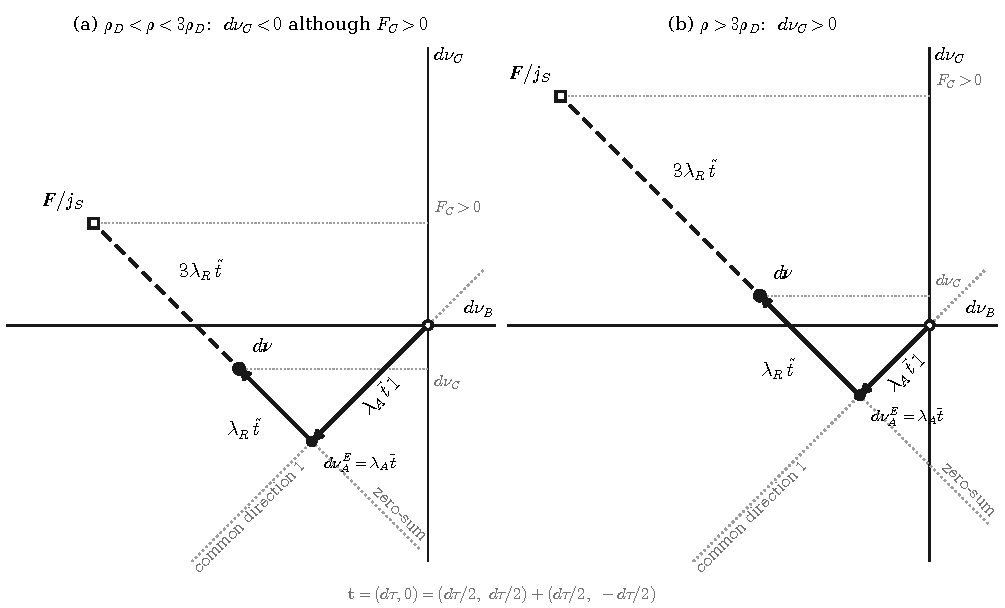
\includegraphics[width=\textwidth]{fig3_decomposition.pdf}
\caption{Average protection and relative treatment at $N=3$. The unilateral tariff $t=(\tau,0)$ is split as $(\tau/2,\tau/2)+(\tau/2,-\tau/2)$. By Theorem~\ref{res:main}, the average-protection component moves both bilateral rates equally along the constant direction $\mathbf{1}$ and carries the whole effective-rate response $d\nu_A^E=\lambda_S\bar t$; the relative-treatment component moves the bilateral rates in opposite directions along the zero-sum direction and leaves the effective rate unchanged. The two components are orthogonal in $(\nu_B,\nu_C)$ space, so the average-protection point is the projection of $\nu$ onto $\mathbf{1}$. Panel (b) shows that the bystander rate $\nu_C$ turns positive once the relative-treatment step dominates, i.e.\ once $\rho>3\rho_1^*$. Drawn at $\alpha_D=0.7$, $\alpha_T=0.6$, $\eta=1.5$, with $\rho=2.2$ in panel (a) and $\rho=5$ in panel (b), so that $\rho_1^*=1.17$ and $3\rho_1^*=3.51$.}
\label{fig:decomposition}
\end{figure}

Theorem~\ref{res:main} also orders bilateral responses directly by tariff treatment. Since $\lambda_D<0$, \eqref{eq:scale-disc} gives $\nu_j-\nu_k=\lambda_D(t_j-t_k)$, so with $\bar t>0$, $t_j>t_k$ implies $\nu_j<\nu_k$, and $A$ depreciates against partner $j$ if and only if
\begin{equation}
\frac{\rho}{N}(\bar t-t_j)>\rho_1^*\,\bar t
\qquad\Longleftrightarrow\qquad
\frac{t_j}{\bar t}<1-\frac{N\rho_1^*}{\rho}.
\label{eq:reltreat}
\end{equation}
Thus $A$ appreciates more against partners facing higher tariffs. Depreciation against a relatively lightly taxed partner requires both $\rho>N\rho_1^*$ and a sufficiently large tariff differential. Appendix~\ref{app:linear} derives \eqref{eq:reltreat} and gives the corresponding responses when $A$ taxes several partners, including a uniform tariff, under which all bilateral rates move together.

\FloatBarrier

\section{Trade Wars and Preferential Tariffs}

\label{sec:wars}

The results above also apply when several countries change tariffs simultaneously. Under symmetry, the bilateral exchange-rate effects can be computed for each tariffing country using Theorem~\ref{res:main} and then added.

\subsection{Trade wars}

\paragraph{Bilateral retaliation.}
Suppose $A$ raises its tariff on $B$ by $d\tau$ and $B$ raises its tariff on $A$ by the same amount. The two effects on the $A$--$B$ rate cancel, while for any bystander $C$,
\begin{equation}
\frac{d\log e_{AB}}{d\tau}\bigg|^{w}=0, \qquad
\frac{d\log e_{AC}}{d\tau}\bigg|^{w}=\frac{\rho-\rho_1^*}{D_N}, \qquad
\frac{d\nu_A^E}{d\tau}\bigg|^{w}=\frac{N-2}{N-1}\frac{\rho-\rho_1^*}{D_N}.
\label{eq:N-war}
\end{equation}

\noindent Relative to a unilateral tariff, retaliation lowers the bystander threshold from $N\rho_1^*$ to $\rho_1^*$. The additional tariff imposed by $B$ affects the $A$--$C$ rate through relative treatment but not through $B$'s average protection. Using \eqref{eq:eigen},
\begin{equation}
\frac{d\log e_{AC}}{d\tau}\bigg|^{w}
=-\frac{\rho_1^*}{D_N}+\frac{\rho}{ND_N}+\frac{(N-1)\rho}{ND_N}
=\frac{\rho-\rho_1^*}{D_N}.
\label{eq:war-components}
\end{equation}
Hence the factor $N$ in the unilateral-tariff threshold disappears under symmetric retaliation.

\paragraph{Global retaliation.}
Suppose instead that $A$ raises its tariff by $d\tau$ on every partner and each partner raises its tariff by $d\tau$ on $A$.

\begin{proposition}[Trade wars]
Under MML:
\begin{enumerate}
\item[(i)] \emph{(Bilateral retaliation.)} In a symmetric bilateral trade war between $A$ and $B$, the belligerents' effective exchange rates depreciate, and every bystander appreciates against both, if and only if $\rho>\rho_1^*$. The threshold is independent of $N$.
\item[(ii)] \emph{(Global retaliation.)} If $A$ taxes every partner and every partner taxes $A$, each at rate $d\tau$, then
\begin{equation}
\frac{d\log e_{Aj}}{d\tau}
=\frac{d\nu_A^E}{d\tau}
=\frac{(N-2)(\rho-\rho_1^*)}{D_N}
\qquad \forall j,
\label{eq:globalwar}
\end{equation}
while all exchange rates among $A$'s partners are unchanged. Hence $A$ depreciates against every partner if and only if $\rho>\rho_1^*$.
\end{enumerate}
\label{res:war}
\end{proposition}

\noindent In (ii) the response vanishes at $N=2$ by symmetry. For $N\geq3$, the same threshold as in the bilateral trade war applies. Retaliation is a genuinely distinct configuration rather than a relabelling of Section~\ref{sec:unilateral}: because each belligerent's own tariff vector is unilateral, the mirror shock contributes to the $A$--$C$ rate through relative treatment on both sides, and the two relative-treatment contributions reinforce rather than offset the average-protection term.

\subsection{The three-country case}

\label{sec:three}

For $N=3$, the unilateral-tariff system can be written explicitly as
\begin{equation}
J=-\frac{mD_3}{4}
\begin{pmatrix}
2 & -1\\
-1 & 2
\end{pmatrix},
\qquad
F=-\frac{m}{4}
\begin{pmatrix}
\rho+\rho_1^*\\
\rho_1^*-\rho
\end{pmatrix},
\qquad
D_3=3\alpha_D(\eta-1)+\rho+1.
\label{eq:3c-JF}
\end{equation}
With $D_3>0$, \eqref{eq:N-slopes}--\eqref{eq:N-slopes-C} at $N=3$ read
\begin{equation}
\frac{d\log e_{AB}}{d\tau}
=-\frac{\rho+3\rho_1^*}{3D_3}<0, \qquad
\boxed{\;\frac{d\log e_{AC}}{d\tau}
=\frac{\rho-3\rho_1^*}{3D_3}\;}, \qquad
\frac{d\log e_{BC}}{d\tau}
=\frac{2\rho}{3D_3}>0.
\label{eq:3c-slopes}
\end{equation}
Thus $A$ appreciates against $B$, $B$ depreciates against $C$, and $A$ depreciates against $C$ if and only if $\rho>3\rho_1^*$. By \eqref{eq:signrule}, $d\nu_C/d\tau\propto F_B+2F_C\propto\rho-3\rho_1^*$, so the sign of $C$'s own disturbance $F_C$, which is positive once $\rho>\rho_1^*$, does not settle the sign of $\nu_C$.

Figure~\ref{fig:threecountry} plots the two equilibrium conditions,
\begin{equation}
\mathrm{TB}_B=0:\quad \nu_C=2\nu_B+\frac{\rho+\rho_1^*}{D_3}d\tau ,
\qquad
\mathrm{TB}_C=0:\quad \nu_C=\tfrac12\nu_B+\frac{\rho-\rho_1^*}{2D_3}d\tau .
\label{eq:3c-loci}
\end{equation}
In the intermediate case $\rho_1^*<\rho<3\rho_1^*$, $C$ gains from trade diversion at unchanged exchange rates and the $\mathrm{TB}_C=0$ locus shifts up. But the larger shift of $\mathrm{TB}_B=0$ drives $\nu_B$ down, and the resulting movement along the upward-sloping $\mathrm{TB}_C=0$ locus more than offsets that shift: $A$ still appreciates against $C$.

\begin{figure}[htbp]
\centering
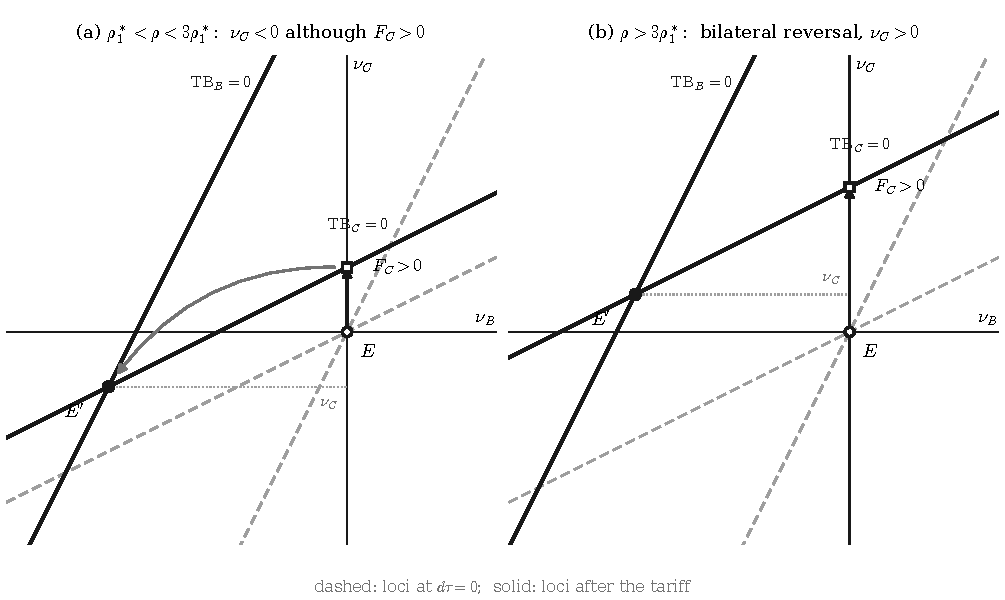
\includegraphics[width=\textwidth]{fig2_three_country.pdf}
\caption{Three-country equilibrium adjustment. The loci are \eqref{eq:3c-loci}; dashed lines are the pre-tariff loci through the initial equilibrium $E$, solid lines the post-tariff loci intersecting at $E'$. The open square is the value of $\nu_C$ that would clear $C$'s trade balance at $\nu_B=0$; the curved arrow in panel~(a) is the subsequent movement along $\mathrm{TB}_C=0$. Panel~(a): $\rho_1^*<\rho<3\rho_1^*$. Panel~(b): $\rho>3\rho_1^*$. Drawn at $\alpha_D=0.7$, $\alpha_T=0.6$, $\eta=1.5$, with $\rho=2.2$ in panel (a) and $\rho=5$ in panel (b), so that $\rho_1^*=1.17$ and $3\rho_1^*=3.51$.}
\label{fig:threecountry}
\end{figure}

\subsection{Competing exporters}

A standard benchmark in the preferential-trade-agreement literature has one importing country and two competing exporters, following Viner (1950) and Mundell (1964). Importer $A$ is endowed only with the numeraire good $y$, while exporters $B$ and $C$ are endowed with good $x$. Preferences are quasilinear, $U_i=u_i(x_i)+y_i$. Country $A$ levies specific tariffs $t_B$ and $t_C$. Let $q_j$ denote exporter $j$'s price and $p$ the domestic price in $A$. Market clearing requires
\begin{equation}
p=q_B+t_B=q_C+t_C, \qquad
M_A(p)=E_B(p-t_B)+E_C(p-t_C), \qquad
M_A'<0, \quad E_j'>0,
\label{eq:pta-mc}
\end{equation}
where $M_A(p)=x_A^d(p)$ and $E_j(q_j)=\omega_j-x_j^d(q_j)$. Differentiating with respect to $t_B$ gives
\begin{equation}
\frac{dp}{dt_B}=\frac{E_B'}{E_B'+E_C'-M_A'}\in(0,1), \qquad
\frac{dq_B}{dt_B}=-\frac{E_C'-M_A'}{E_B'+E_C'-M_A'}<0, \qquad
\frac{dq_C}{dt_B}=\frac{dp}{dt_B}>0.
\label{eq:pta-cs}
\end{equation}

\begin{proposition}[Competing-exporter terms-of-trade effect]
A tariff on imports from $B$ worsens $B$'s terms of trade and improves $C$'s terms of trade.
\label{res:viner}
\end{proposition}

\subsection{Preferential tariffs}

The competing-exporter result provides a useful comparison with the three-country case of our model. An improvement in $C$'s terms of trade corresponds to an increase in $e_{AC}$ by \eqref{eq:rer}. In the competing-exporter model this occurs unconditionally after a tariff on $B$, whereas in our model \eqref{eq:3c-slopes} requires
\begin{equation*}
\rho>3\rho_1^*.
\end{equation*}

The difference reflects the economic environment. In the competing-exporter model, $A$ does not produce the importable good, so a tariff reallocates demand between the two foreign suppliers without inducing substitution toward a domestically produced import-competing good. In our model, both margins are present: substitution between domestic and imported goods, governed by $\eta$, and substitution across foreign import origins, governed by $\rho$. The terms-of-trade effect on a third country therefore depends on their relative strength.

A preferential tariff reduction gives the corresponding result with the signs reversed. Suppose $A$ lowers its tariff on $B$ alone, so that $t=-\tau\,\mathbf{e}_B$. For a non-member $C$, Theorem~\ref{res:main} implies that $C$'s terms of trade worsen if and only if
\begin{equation*}
\rho>N\rho_1^*.
\end{equation*}
Thus our model produces the same sign as the standard competing-exporter result only when substitution across foreign origins is sufficiently strong relative to the other general-equilibrium effects.

The two environments are not formally nested. The competing-exporter model has a common importable supplied by $B$ and $C$ and quasilinear preferences, while our model has country-specific differentiated tradables and nested-CES preferences. The comparison is therefore one of mechanisms. The competing-exporter model isolates substitution across foreign suppliers, whereas our framework also includes substitution between domestic and imported goods and the associated income effects.

At $N=3$, the threshold can be written as
\begin{equation}
\rho_3^*=3\rho_1^*=3+3\alpha_D(\eta-1)-3\alpha_T(1-\alpha_D).
\label{eq:pta-decomp}
\end{equation}
The threshold rises with the domestic-import substitution term and falls with the import share. This helps explain why the third-country terms-of-trade effect is unambiguous in the competing-exporter benchmark but can change sign in the nested-CES model.

Competing-exporter models such as Bagwell and Staiger (1999) and Ornelas (2005) abstract from trade between the foreign suppliers and use quasilinear preferences, while bloc and endowment models such as Krugman (1991) and Bond and Syropoulos (1996) abstract from domestic production of the importable. Kemp and Wan (1976) consider a more general customs-union environment. The comparison here is not intended to nest these models, but to identify which additional margins determine the sign of third-country terms-of-trade effects in our setting.

\section{Conclusion}

A tariff affects exchange rates through two steps. At unchanged exchange rates it changes countries' trade balances, summarized by $F$; exchange rates then adjust through $(-J)^{-1}$. In the two-country case this reduces to the familiar Marshall--Lerner result: under the elasticity condition, a tariff appreciates the tariffing country's currency.

With three or more countries, a tariff can also redirect expenditure across foreign suppliers. The tariffing country therefore continues to appreciate against the targeted partner, but its exchange rate against an untariffed partner can move in either direction. Under symmetry, the response to any tariff vector separates into an average-protection component and a relative-treatment component. Average protection determines the effective exchange-rate response, while relative treatment determines deviations of bilateral rates from that common response.

For a unilateral tariff on one partner, the tariffing country's effective exchange rate always appreciates under MML. Its bilateral rate against an untariffed bystander reverses only if
\[
\rho>N\rho_1^*.
\]
The corresponding trade-balance effect on the bystander changes sign already at $\rho>\rho_1^*$, a threshold that is itself independent of $N$. In the nested-CES benchmark, the difference comes from multilateral exchange-rate adjustment rather than from any dilution of trade diversion: the relative strength of the two tariff disturbances, $g_D/g_S=\rho/\rho_1^*$, does not depend on $N$, while $j_D/j_S=N$. Under the symmetric nested-CES benchmark, a given relative exchange-rate movement has $N$ times the trade-balance effect of a common movement, so a given relative trade-balance disturbance requires only $1/N$ as much exchange-rate adjustment.

Other tariff configurations alter this comparison. Under symmetric bilateral retaliation, the bystander threshold falls to $\rho_1^*$ and is independent of $N$. In the standard competing-exporter benchmark, substitution across foreign suppliers generates an unambiguous third-country terms-of-trade effect; in our model, that effect interacts with domestic-import substitution and income effects and therefore need not have an unconditional sign.

The main implication is that the familiar two-country exchange-rate result survives multilateralization most cleanly at the level of the effective exchange rate. Bilateral exchange rates also reflect how trade policy differs across partners, and their responses need not inherit the sign of the aggregate adjustment.

\section*{References}

\begingroup
\setlength{\parindent}{0pt}
\newcommand{\refentry}[1]{\par\hangindent=1.5em\hangafter=1 #1\par\vspace{2pt}}

\refentry{Bagwell, Kyle, and Robert W. Staiger (1999). ``An Economic Theory of GATT.'' \emph{American Economic Review} 89(1), 215--248.}

\refentry{Bond, Eric W., and Costas Syropoulos (1996). ``The Size of Trading Blocs: Market Power and World Welfare Effects.'' \emph{Journal of International Economics} 40(3--4), 411--437.}

\refentry{Kemp, Murray C., and Henry Y. Wan (1976). ``An Elementary Proposition Concerning the Formation of Customs Unions.'' \emph{Journal of International Economics} 6(1), 95--97.}

\refentry{Krugman, Paul (1991). ``Is Bilateralism Bad?'' In Elhanan Helpman and Assaf Razin (eds.), \emph{International Trade and Trade Policy}, 9--23. Cambridge, MA: MIT Press.}

\refentry{Mundell, Robert A. (1964). ``Tariff Preferences and the Terms of Trade.'' \emph{The Manchester School of Economic and Social Studies} 32(1), 1--13.}

\refentry{Ornelas, Emanuel (2005). ``Trade Creating Free Trade Areas and the Undermining of Multilateralism.'' \emph{European Economic Review} 49(7), 1717--1735.}

\refentry{Viner, Jacob (1950). \emph{The Customs Union Issue}. New York: Carnegie Endowment for International Peace.}

\endgroup

\appendix

\section{Exact Cobb--Douglas solution ($N = 2$)}

\label{app:cd}

At $\eta = 1$, expenditure shares are fixed at their weights. From \eqref{eq:income}, $I_A = w_A L_A/[1 - \tfrac{\tau}{1+\tau}m]$, and $\mathrm{TB}_A = 0$ becomes $e\,m\,w_B L_B = m I_A/(1+\tau)$:
\begin{equation}
e(\tau) = \frac{w_A L_A}{w_B L_B}\cdot \frac{1}{1 + (1-m)\tau},
\qquad
\frac{d\log e}{d\tau}\bigg|_{\tau=0} = -(1-m) = -\frac{\rho_1^*}{D_2}\bigg|_{\eta=1}.
\label{eq:2c-exact}
\end{equation}
Thus $e(\tau)$ is decreasing in $\tau$, so the sign of the linearized response in \eqref{eq:2c-slope} is exact for all tariff levels in this case. Here $\eta = 1$ fixes the elasticity, not the weight $\alpha_D$.

\section{The Linearized System}

\label{app:linear}

At the balanced free-trade baseline, let $m\equiv\alpha_T(1-\alpha_D)$, $b_{ij}\equiv\beta_{ij}$, and $f_{ij}=s_{ij}\widetilde I_i$, with $\sum_k f_{ki}=\sum_j f_{ij}$. All incomes and flows are measured in the common currency. Linearizing the demand, income, and trade-balance equations gives
\begin{align}
dp_{ij} &= \nu_j-\nu_i+dt_{ij} \qquad (dp_{ii}=0), \label{eq:dp}\\
d\log P_{M_i} &= \sum_{j\neq i}b_{ij}\,dp_{ij}, \qquad
d\log P_{T_i}=(1-\alpha_D)\,d\log P_{M_i}, \label{eq:dindex}\\
d\log s_{ii} &= -(1-\eta)(1-\alpha_D)\,d\log P_{M_i}, \label{eq:dshome}\\
d\log s_{ij} &= (1-\rho)\big(dp_{ij}-d\log P_{M_i}\big)
+(1-\eta)\alpha_D\,d\log P_{M_i}, \label{eq:dsfor}\\
d\log\widetilde I_i &= \nu_i+\sum_{j\neq i}s_{ij}\,dt_{ij}, \label{eq:dincome}\\
d\,\mathrm{TB}_i &= \sum_{k\neq i}f_{ki}\big(d\log s_{ki}+d\log\widetilde I_k-dt_{ki}\big)
-\sum_{j\neq i}f_{ij}\big(d\log s_{ij}+d\log\widetilde I_i-dt_{ij}\big).
\label{eq:dtb}
\end{align}
These equations determine the model-specific matrices $J$ and $G$ in \eqref{eq:JFdef}. At $N=2$ they reduce to the calculation in Section~\ref{sec:twocountry}.

At the symmetric baseline, every off-diagonal element of the full $N\times N$ exchange-rate Jacobian is
\begin{equation}
\widetilde J_{il}=\frac{m}{(N-1)^2}D_N \quad (l\neq i), \qquad
D_N\equiv N\alpha_D(\eta-1)+(N-2)\rho+1.
\label{eq:full-jacobian}
\end{equation}
Lemma~\ref{lem:fulljac} below gives the derivation. MML holds if and only if $D_N>0$. In particular,
\begin{equation*}
\eta\geq1 \quad\Longrightarrow\quad D_N>0
\quad\Longleftrightarrow\quad \text{MML \eqref{eq:invpos} under symmetry}.
\end{equation*}
Thus $D_N$ is the $N$-country counterpart of the two-country adjustment coefficient $D_2=\varepsilon_X+\varepsilon_M-1$.

\begin{lemma}[Full Jacobian at the symmetric baseline]
At the symmetric balanced baseline of Appendix~\ref{app:linear}, where $b_{ij}=1/(N-1)$ and $f_{ij}=m/(N-1)$, the full $N\times N$ Jacobian of the nested-CES model is
\begin{equation*}
\widetilde J_{il} = \frac{m}{(N-1)^2}D_N
\quad
(l\neq i),
\qquad
\widetilde J_{ii} = -\frac{m}{N-1}D_N,
\qquad
D_N = N\alpha_D(\eta-1)+(N-2)\rho+1.
\end{equation*}
\label{lem:fulljac}
\end{lemma}

\begin{proof}
Set $dt_{jk}=0$, so $dp_{ij}=\nu_j-\nu_i$ and $d\log\widetilde I_i=\nu_i$. Writing $S\equiv\sum_j\nu_j$, \eqref{eq:dindex} gives
\[
d\log P_{M_k} = \frac{S-N\nu_k}{N-1},
\qquad
\frac{\partial\,d\log P_{M_k}}{\partial\nu_l} = \frac{1-N\delta_{kl}}{N-1}.
\]
On the import side,
\[
\sum_{j\neq i} \big( dp_{ij}-d\log P_{M_i} \big) = 0,
\]
so the $(1-\rho)$ terms cancel when \eqref{eq:dsfor} is summed over $j\neq i$. Thus,
\[
\sum_{j\neq i}d\log s_{ij} = (N-1)(1-\eta)\alpha_D\,d\log P_{M_i}.
\]
Substituting into \eqref{eq:dtb} gives
\[
d\,\mathrm{TB}_i = \frac{m}{N-1} \Big[ \sum_{k\neq i} \big( d\log s_{ki}+\nu_k \big) - (N-1)(1-\eta)\alpha_D\,d\log P_{M_i} - (N-1)\nu_i \Big].
\]
Fix $l\neq i$ and differentiate term by term:
\[
\frac{\partial}{\partial\nu_l} \sum_{k\neq i}d\log s_{ki} = -(1-\rho)\frac{N-2}{N-1} - \frac{(1-\eta)\alpha_D}{N-1}.
\]
The export income terms contribute one, the import-side price-index term contributes $-(1-\eta)\alpha_D$, and the import income term contributes zero. Collecting terms gives
\[
\widetilde J_{il} = \frac{m}{(N-1)^2} \Big[ (N-1) - (1-\rho)(N-2) + N\alpha_D(\eta-1) \Big] = \frac{m}{(N-1)^2}D_N.
\]
The diagonal follows from \eqref{eq:hom}:
\[
\widetilde J_{ii} = -(N-1)\widetilde J_{il} = -\frac{m}{N-1}D_N.
\]
At $N=2$ this gives $\widetilde J_{AB}=mD_2$, the coefficient in \eqref{eq:2c-collected}; deleting row and column $A$ at $N=3$ reproduces $J$ in \eqref{eq:3c-JF}.
\end{proof}

\paragraph{The two-country case.}
At the balanced free-trade baseline with normalized incomes, $s_{AB}=s_{BA}=m$. At $N=2$ each country has a single import origin, so $dp_{AB} = d\log P_{M_A} = \nu_B + d\tau$ and $dp_{BA} = d\log P_{M_B} = -\nu_B$. Log-differentiating \eqref{eq:sfor} and \eqref{eq:income}, with incomes in the common currency,
\[
\begin{aligned}
d\log s_{AB} &= (1-\eta)\alpha_D(\nu_B+d\tau),
&\qquad
d\log s_{BA} &= -(1-\eta)\alpha_D\,\nu_B,\\
d\log \widetilde I_A &= m\,d\tau,
&\qquad
d\log \widetilde I_B &= \nu_B .
\end{aligned}
\]
Substituting into \eqref{eq:tb} and using that the tariff wedge lowers the border value of $A$'s imports by $d\tau$,
\[
d\,\mathrm{TB}_A = m\Big[\big(1+2\alpha_D(\eta-1)\big)\nu_B + \big(1-m+\alpha_D(\eta-1)\big)d\tau\Big] ,
\]
which is \eqref{eq:2c-collected}, with $D_2=1+2\alpha_D(\eta-1)$ and $\rho_1^*=1-m+\alpha_D(\eta-1)$, and \eqref{eq:2c-slope} follows. For the elasticity form, hold income fixed and let $M(p)$ denote import volume at consumer price $p=p_{AB}$. Since import value is $s_{AB}I_A$,
\[
\varepsilon_M \equiv -\frac{\partial\log M}{\partial\log p} = 1-\frac{\partial\log s_{AB}}{\partial\log p} = 1-(1-\eta)\alpha_D = 1+\alpha_D(\eta-1).
\]
By symmetry, $\varepsilon_X=1+\alpha_D(\eta-1)$. Differentiating $\mathrm{TB}_A(e,\tau)=X(1/e)-e\,M((1+\tau)e)$ at $\tau=0$ and using balanced trade, $X=eM$, gives
\[
\frac{\partial\mathrm{TB}_A}{\partial e} = M(\varepsilon_X+\varepsilon_M-1).
\]
Hence $\varepsilon_X+\varepsilon_M-1=2\alpha_D(\eta-1)+1=D_2$, so the stability condition $D_2>0$ is exactly $\varepsilon_X+\varepsilon_M>1$. Since $\rho_1^*>0$ by \eqref{eq:rho1-identity}, the slope $-\rho_1^*/D_2$ is negative whenever $D_2>0$.


\paragraph{The tariff disturbance and the four eigenvalues.}
At unchanged exchange rates, the effect on partner $i$'s trade balance follows from \eqref{eq:dtb}. Since only $i$'s exports to $A$ are directly affected,
\begin{equation}
d\,\mathrm{TB}_i\big|_{\nu\ \mathrm{fixed}}
=f_{Ai}\big(d\log s_{Ai}+d\log\widetilde I_A-t_i\big)
=\frac{m}{N-1}\Big[-\rho_1^*\,\bar t-\rho\,(t_i-\bar t)\Big].
\label{eq:impact-chain}
\end{equation}
Reading off the coefficients on $\bar t$ and $\tilde t_i$ gives the tariff-effect eigenvalues \eqref{eq:g-eigen}. Deleting row and column $A$ from \eqref{eq:full-jacobian} gives the exchange-rate adjustment matrix
\begin{equation}
-J=c\big(NI-\mathbf{1}\mathbf{1}'\big), \qquad
c\equiv\frac{mD_N}{(N-1)^2},
\label{eq:J-matrix}
\end{equation}
whose eigenvalues are $j_S=c$ on $\operatorname{span}\{\mathbf 1\}$ and $j_D=Nc$ on the zero-sum subspace, which is \eqref{eq:j-eigen}. Dividing \eqref{eq:g-eigen} by \eqref{eq:j-eigen} gives \eqref{eq:eigen}.

\paragraph{Direct derivation of \eqref{eq:N-slopes}.}
The unilateral slopes can also be obtained by inverting a reduced two-equation system. Since the equilibrium is unique under MML and the system is invariant to permutations of the $N-2$ bystanders, all bystanders have the same response $\nu_C$. The equilibrium therefore reduces to the conditions for $B$ and one representative bystander.

Equations \eqref{eq:dp}--\eqref{eq:dindex} give
\begin{equation}
d\log P_{M_A} = \frac{\nu_B+d\tau+(N-2)\nu_C}{N-1},
\qquad
d\log P_{M_B} = \frac{(N-2)\nu_C}{N-1}-\nu_B,
\qquad
d\log P_{M_C} = \frac{\nu_B-2\nu_C}{N-1}.
\label{eq:N-indices}
\end{equation}
Also,
\[
d\log\widetilde I_A = \frac{m}{N-1}d\tau,
\qquad
d\log\widetilde I_B = \nu_B,
\qquad
d\log\widetilde I_C = \nu_C.
\]
The deviations of bilateral prices from the corresponding import indices are
\[
\begin{aligned}
dp_{AB}-d\log P_{M_A}
&=
\tfrac{N-2}{N-1}
(\nu_B+d\tau-\nu_C),
&
dp_{AC}-d\log P_{M_A}
&=
\tfrac{1}{N-1}
(\nu_C-\nu_B-d\tau),\\
dp_{BA}-d\log P_{M_B}
&=
-\tfrac{N-2}{N-1}\nu_C,
&
dp_{BC}-d\log P_{M_B}
&=
\tfrac{1}{N-1}\nu_C,\\
dp_{CA}-d\log P_{M_C}
&=
-\tfrac{1}{N-1}
\big[
(N-3)\nu_C+\nu_B
\big],
&
dp_{CC'}-d\log P_{M_C}
&=
\tfrac{1}{N-1}
(2\nu_C-\nu_B),\\
dp_{CB}-d\log P_{M_C}
&=
\tfrac{1}{N-1}
\big[
(N-2)\nu_B-(N-3)\nu_C
\big]. &&
\end{aligned}
\]
Using \eqref{eq:dsfor} and flow values $m/(N-1)$, collecting the two trade-balance conditions gives
\begin{equation}
D_N
\begin{pmatrix}
-(N-1) & N-2\\
1 & -2
\end{pmatrix}
\begin{pmatrix}
\nu_B\\
\nu_C
\end{pmatrix}
=
\begin{pmatrix}
(N-2)\rho+\rho_1^*\\
\rho_1^*-\rho
\end{pmatrix}
d\tau,
\qquad
D_N
=
N\alpha_D(\eta-1)+(N-2)\rho+1.
\label{eq:N-system}
\end{equation}
The matrix has determinant $N$, so inversion gives \eqref{eq:N-slopes}. At $N=3$ this reduces to \eqref{eq:3c-slopes}, and at $N=2$ to \eqref{eq:2c-slope}.

\paragraph{Derivation of \eqref{eq:N-slopes}--\eqref{eq:Nthresh}.}
By Theorem~\ref{res:main},
\[
\nu = \lambda_S\bar t\,\mathbf{1} + \lambda_D\tilde t.
\]
For $t=d\tau\,\mathbf{e}_B$,
\[
\bar t = \frac{d\tau}{N-1},
\qquad
\tilde t_C = -\frac{d\tau}{N-1},
\]
so
\[
\nu_C = \frac{\lambda_S-\lambda_D}{N-1}d\tau = \frac{\rho-N\rho_1^*}{ND_N}d\tau.
\]
Under MML, $D_N>0$, so
\[
\operatorname{sign} \frac{d\log e_{AC}}{d\tau} = \operatorname{sign} (\rho-N\rho_1^*).
\]
The same substitution with
\[
\tilde t_B = \frac{N-2}{N-1}d\tau
\]
gives the remaining expressions in \eqref{eq:N-slopes}.


\paragraph{Derivation of \eqref{eq:N-neer}.}
By Theorem~\ref{res:main},
\[
d\nu_A^E = \lambda_S\bar t
\]
with symmetric weights $w_{Aj}=1/(N-1)$. For $t=d\tau\,\mathbf{e}_B$,
\[
\bar t = \frac{d\tau}{N-1},
\]
so
\[
\frac{d\nu_A^E}{d\tau} = \frac{\lambda_S}{N-1} = -\frac{\rho_1^*}{D_N}.
\]
By \eqref{eq:rho1-identity}, $\rho_1^*>0$, while $D_N>0$ under MML. The response is therefore negative for every $N\geq2$ and every admissible $\rho$.


\paragraph{Derivation of \eqref{eq:single}.}
With $\rho=\eta=\sigma$,
\[
N\rho_1^* = N\big[ 1+\alpha_D(\sigma-1)-\alpha_T(1-\alpha_D) \big],
\]
so
\[
N\rho_1^*-\sigma = \sigma(N\alpha_D-1) + N(1-\alpha_D)(1-\alpha_T).
\]
For $\alpha_D\geq1/N$ both terms are nonnegative, with both zero only at $\alpha_D=1/N$, $\alpha_T=1$; hence $\rho=\sigma\leq N\rho_1^*$. Since $\rho_1^*$ does not involve $\rho$,
\[
N\rho_1^*-\eta = \eta(N\alpha_D-1) + N(1-\alpha_D)(1-\alpha_T).
\]
At $\alpha_D=1/N$,
\[
N\rho_1^*-\sigma = (N-1)(1-\alpha_T),
\qquad
D_N = (N-1)\sigma,
\]
so by \eqref{eq:N-slopes-C},
\[
\frac{d\log e_{AC}}{d\tau} = -\frac{1-\alpha_T}{N\sigma}.
\]

\paragraph{Derivation of \eqref{eq:reltreat}.}
From \eqref{eq:scale-disc},
\[
\nu_j-\nu_k = \lambda_D(t_j-t_k),
\]
and $\lambda_D<0$, proving the ordering result. Moreover,
\[
\nu_j>0
\]
if and only if
\[
\lambda_S\bar t + \lambda_D(t_j-\bar t) > 0.
\]
Substituting \eqref{eq:eigen} and dividing by $(N-1)/D_N>0$ gives
\[
-\rho_1^*\bar t - \frac{\rho}{N}(t_j-\bar t) > 0,
\]
or
\[
\frac{\rho}{N}(\bar t-t_j) > \rho_1^*\bar t.
\]
For $\bar t>0$, this is equivalent to
\[
\frac{t_j}{\bar t} < 1-\frac{N\rho_1^*}{\rho}.
\]
The right-hand side is positive only if $\rho>N\rho_1^*$.


\paragraph{Tariffs on several partners.}
If $A$ raises its tariff by $\tau$ on a set of $k$ partners, $1\leq k\leq N-1$, then for every untargeted partner $C$ and every targeted partner $B$,
\begin{equation}
\frac{d\log e_{AC}}{\tau}=\frac{k(\rho-N\rho_1^*)}{ND_N}, \qquad
\frac{d\log e_{AB}}{\tau}=-\frac{k\rho_1^*}{D_N}-\frac{(N-1-k)\rho}{ND_N}, \qquad
\frac{d\nu_A^E}{\tau}=-\frac{k\rho_1^*}{D_N}.
\label{eq:k-targets}
\end{equation}
For every $k\leq N-2$, the bystander response has the same threshold $\rho>N\rho_1^*$. When all partners face the same tariff,
\begin{equation}
\frac{d\log e_{Aj}}{d\tau}
=-\frac{(N-1)\rho_1^*}{D_N}
=\frac{d\nu_A^E}{d\tau}
\qquad \forall j.
\label{eq:N-broad}
\end{equation}
All bilateral rates then move together, and substitution across foreign origins plays no role.

To derive these, let $t_j=\tau$ on the $k$ targets and zero otherwise, so that
\[
\bar t = \frac{k\tau}{N-1},
\qquad
\tilde t_B = \frac{N-1-k}{N-1}\tau
\]
for a target, and
\[
\tilde t_C = -\frac{k\tau}{N-1}
\]
for a bystander. Substituting into \eqref{eq:scale-disc} gives
\[
\nu_C = \frac{k\tau}{N-1} (\lambda_S-\lambda_D) = \frac{k\tau}{ND_N} (\rho-N\rho_1^*),
\]
together with the target and NEER responses in \eqref{eq:k-targets}. For every $k\leq N-2$, the sign of the bystander response is therefore determined by $\rho-N\rho_1^*$. At $k=N-1$ there is no bystander and $\tilde t=0$, giving \eqref{eq:N-broad}.


\paragraph{The three-country system.}
At $N=3$, \eqref{eq:dp}--\eqref{eq:dindex} give
\begin{equation*}
d\log P_{M_A} = \tfrac12(\nu_B+\nu_C+d\tau),
\qquad
d\log P_{M_B} = \tfrac12\nu_C-\nu_B,
\qquad
d\log P_{M_C} = \tfrac12\nu_B-\nu_C.
\end{equation*}
Also,
\[
d\log\widetilde I_A = \tfrac{m}{2}d\tau,
\qquad
d\log\widetilde I_B = \nu_B,
\qquad
d\log\widetilde I_C = \nu_C.
\]
The deviations of bilateral prices from the corresponding import indices are
\[
\begin{aligned}
dp_{AB}-d\log P_{M_A}
&=
\tfrac12(\nu_B-\nu_C+d\tau),
&
dp_{AC}-d\log P_{M_A}
&=
\tfrac12(\nu_C-\nu_B-d\tau),\\
dp_{BA}-d\log P_{M_B}
&=
-\tfrac12\nu_C,
&
dp_{BC}-d\log P_{M_B}
&=
\tfrac12\nu_C,\\
dp_{CA}-d\log P_{M_C}
&=
-\tfrac12\nu_B,
&
dp_{CB}-d\log P_{M_C}
&=
\tfrac12\nu_B.
\end{aligned}
\]
The share changes then follow from \eqref{eq:dsfor}. With flow values $m/2$, \eqref{eq:dtb} gives
\[
\begin{aligned}
\tfrac{2}{m}\,d\,\mathrm{TB}_B
&=
\big(
d\log s_{AB}+\tfrac{m}{2}d\tau-d\tau
\big)
+
\big(
d\log s_{CB}+\nu_C
\big)
-
\big(
d\log s_{BA}+\nu_B
\big)
-
\big(
d\log s_{BC}+\nu_B
\big),\\
\tfrac{2}{m}\,d\,\mathrm{TB}_C
&=
\big(
d\log s_{AC}+\tfrac{m}{2}d\tau
\big)
+
\big(
d\log s_{BC}+\nu_B
\big)
-
\big(
d\log s_{CA}+\nu_C
\big)
-
\big(
d\log s_{CB}+\nu_C
\big).
\end{aligned}
\]
For example, the coefficient on $\nu_B$ in $\tfrac{2}{m}d\,\mathrm{TB}_B$ is
\[
\tfrac12\big[(1-\rho)+(1-\eta)\alpha_D\big] + \tfrac12\big[(1-\rho)+(1-\eta)\alpha_D\big] + 2(1-\eta)\alpha_D-2 = -D_3.
\]
Collecting the remaining coefficients gives \eqref{eq:3c-JF}, and inverting gives \eqref{eq:3c-slopes}. With $D_3>0$, the numerator for $e_{AB}$ is negative and the numerator for $e_{BC}$ is positive. The bystander response satisfies
\[
\operatorname{sign} \frac{d\log e_{AC}}{d\tau} = \operatorname{sign} (\rho-3\rho_1^*).
\]


\section{Real exchange rates}

\label{app:real}

This appendix gives the real exchange-rate counterparts of the results in Sections~\ref{sec:scaledisc}--\ref{sec:unilateral}.

From \eqref{eq:rer} and \eqref{eq:indices},
\begin{equation*}
d\log q_{Aj} = \nu_j + \alpha_T \big( d\log P_{T_j}^{\mathrm{own}} - d\log P_{T_A}^{\mathrm{own}} \big).
\end{equation*}
For a tariff vector $t$, symmetry implies
\[
d\log P_{M_A} = d\nu_A^E+\bar t,
\qquad
d\log P_{M_j} = d\nu_A^E-\frac{N}{N-1}\nu_j
\]
for a partner that imposes no tariff. Hence
\begin{equation}
\begin{aligned}
d\log q_{Aj} &= \Big(1-\frac{mN}{N-1}\Big)\nu_j - m\,\bar t,\\
dq_A^E &= \Big[\Big(1-\frac{mN}{N-1}\Big)\lambda_S-m\Big]\bar t,\\
d\log q_{Aj}-dq_A^E &= \Big(1-\frac{mN}{N-1}\Big)\lambda_D\,\tilde t_j.
\end{aligned}
\label{eq:q-decomp}
\end{equation}
Thus average protection determines the real effective exchange-rate response, while relative treatment determines bilateral deviations around it, subject to the price-index adjustment in \eqref{eq:q-decomp}.

For a unilateral tariff, $\bar t=d\tau/(N-1)$ and
\begin{equation}
d\log q_{Aj} = \Big(1-\frac{mN}{N-1}\Big)\nu_j - \frac{m}{N-1}\,d\tau,
\qquad
j=B,C.
\label{eq:qgen}
\end{equation}
Setting $d\log q_{AC}=0$ and using \eqref{eq:N-slopes}, for $m<1/N$,
\begin{equation}
\rho_q^*(N) = \frac{ \big[(N-1)-mN\big]\,N\rho_1^* + mN\big[N\alpha_D(\eta-1)+1\big] }{ (N-1)(1-mN) } \;>\; N\rho_1^*.
\label{eq:N-rhoq}
\end{equation}
Averaging \eqref{eq:qgen} gives
\begin{equation}
\frac{dq_A^E}{d\tau} = -\Big(1-\frac{mN}{N-1}\Big)\frac{\rho_1^*}{D_N} - \frac{m}{N-1} \;<\; 0
\qquad
\text{for all } \rho,N \ \big(m<\tfrac{N-1}{N}\big).
\label{eq:N-reer}
\end{equation}

\begin{proposition}[Real exchange rates]
Under MML, (i) the real bilateral reversal threshold exceeds the nominal threshold, $\rho_q^*(N)>N\rho_1^*$, and (ii) the REER appreciates for every $\rho$ and $N$, $dq_A^E/d\tau<0$.
\label{res:real}
\end{proposition}

\noindent Both results reflect the direct price-index effect of the tariff. At a given nominal exchange rate, the tariff raises $A$'s consumer prices, making a real bilateral depreciation harder to obtain and reinforcing the effective appreciation.

\section{Asymmetry}

\label{app:asym}

The disturbance-adjustment representation \eqref{eq:system} and MML \eqref{eq:invpos} do not require symmetry, and at any balanced baseline the linearized system \eqref{eq:dp}--\eqref{eq:dtb} continues to hold with baseline shares and incomes as coefficients: $b_{ij}$, the share of origin $j$ in $i$'s import bundle; $h_i$, the home share of $i$'s tradable expenditure; and $y_i\equiv\widetilde I_i$, $i$'s income in the common currency. What requires symmetry is the collapse of the response to the two coefficients $\lambda_S$ and $\lambda_D$ of Proposition~\ref{res:decomp}. Away from symmetry, $G$ and $-J$ generally no longer act separately on average protection and relative treatment, so changes in relative treatment can affect the effective exchange rate, and the closed-form thresholds of Section~\ref{sec:symmetric} need not survive. This appendix records what does.

\paragraph{Bilateral thresholds.}
The elasticity $\rho$ enters the share responses \eqref{eq:dsfor} only through $(1-\rho)$, so every entry of $J$ and $F$ is linear in $\rho$. Each entry of $\operatorname{adj}(-J)$ is therefore a polynomial of degree at most $N-2$ in $\rho$, and each numerator $[\operatorname{adj}(-J)F]_i$ in \eqref{eq:system} a polynomial of degree at most $N-1$. Since $\det(-J)>0$ under MML, a bilateral response can change sign only at a root of this numerator. Symmetry reduces the problem to the two coefficients of Proposition~\ref{res:decomp}, yielding the linear thresholds \eqref{eq:Nthresh} and \eqref{eq:3c-slopes}. At a general asymmetric baseline the $N=3$ numerator is already quadratic in $\rho$:
\begin{equation}
\operatorname{sign}\frac{d\log e_{AC}}{d\tau} = \operatorname{sign} \big( c_2\rho^2+c_1\rho+c_0 \big),
\qquad
c_2 = b_{AB}b_{AC}b_{CA}b_{CB} (1-h_A)(1-h_C)y_Ay_C.
\label{eq:asym-quad}
\end{equation}
The coefficients $c_1$ and $c_0$ depend on the full pattern of trade shares and country sizes. Provided MML continues to hold, $c_2>0$ whenever $A$ and $C$ each import from both foreign origins, so sufficiently strong substitution across import origins still reverses $e_{AC}$. The relevant threshold is the largest positive root; it equals $3\rho_1^*$ at the symmetric point, but away from symmetry there is no universal bilateral threshold, and for $N\geq4$ a response may change sign more than once as $\rho$ varies.

\paragraph{The effective exchange rate.}
Let the target receive a multiple $\kappa$ of its symmetric bilateral import share, $b_{AB}=b_{BA}=\kappa/(N-1)$, with the remaining shares chosen so that trade stays balanced and the bystanders stay interchangeable, and use NEER weights $w_{Aj}=b_{Aj}$; $\kappa=1$ is the symmetric benchmark. If $\kappa\geq1$, the effective rate appreciates for every $\rho$ once $N$ is sufficiently large. If $\kappa<1$, it depreciates for $\rho$ above a threshold of order $N\rho_1^*/(1-\kappa)$: when the target receives less than its symmetric trade weight, depreciations against the bystanders can outweigh the appreciation against the target. The unconditional NEER appreciation of Section~\ref{sec:unilateral} therefore need not survive asymmetric trade weights; no claim is made for arbitrary asymmetric trade networks.

\section{Correspondence across $N$}

\label{app:table}

\begin{center}
\begin{tabular}{p{3.6cm}p{3.0cm}p{3.4cm}p{4.2cm}}
\toprule
object & $N=2$ & $N=3$ & general $N$ \\
\midrule
adjustment condition & $\varepsilon_X+\varepsilon_M-1=D_2>0$ & $D_3>0$ & MML: $-J$ a nonsingular M-matrix \\[3pt]
sufficient primitive condition & $\eta\geq1$ & $\eta\geq1$ & gross substitutability (Assumption~\ref{as:gs}) \\[3pt]
sign rule & scalar response & weights $\tfrac{1}{3}\left(\begin{smallmatrix}2&1\\1&2\end{smallmatrix}\right)$ & $\operatorname{sign}\big(\sum_j\vartheta_{ij}F_j\big)$, $\vartheta\geq0$ \\[3pt]
adjustment eigenvalues $j_S,j_D$ \eqref{eq:j-eigen} & $mD_2$, --- & $mD_3/4$, $3mD_3/4$ & $mD_N/(N-1)^2$, $NmD_N/(N-1)^2$ \\[3pt]
tariff-effect eigenvalues $g_S,g_D$ \eqref{eq:g-eigen} & $-m\rho_1^*$, --- & $-m\rho_1^*/2$, $-m\rho/2$ & $-m\rho_1^*/(N-1)$, $-m\rho/(N-1)$ \\[3pt]
disturbance vs.\ adjustment ratios \eqref{eq:gj-ratios} & --- & $\tfrac{g_D}{g_S}=\tfrac{\rho}{\rho_1^*}$, $\tfrac{j_D}{j_S}=3$ & $\tfrac{g_D}{g_S}=\tfrac{\rho}{\rho_1^*}$ (free of $N$), $\tfrac{j_D}{j_S}=N$ \\[3pt]
bilateral reversal threshold & none & $3\rho_1^*$ & $N\rho_1^*$ under symmetry; polynomial roots in general \\[3pt]
real bilateral threshold & none & $\rho_q^*(3)$ & $\rho_q^*(N)$ \eqref{eq:N-rhoq} \\[3pt]
NEER, unilateral tariff & $-\rho_1^*/D_2$ & $-\rho_1^*/D_3$ & $-\rho_1^*/D_N$ under symmetry \\[3pt]
response coefficients $\lambda_S,\lambda_D$ \eqref{eq:eigen} & $-\rho_1^*/D_2$, --- & $-2\rho_1^*/D_3$, $-2\rho/(3D_3)$ & $-(N-1)\rho_1^*/D_N$, $-(N-1)\rho/(ND_N)$ \\[3pt]
trade-war threshold & --- & $\rho_1^*$ & $\rho_1^*$, independent of $N$ \\
\bottomrule
\end{tabular}
\end{center}

\section{Proofs}

\label{app:proofs}

Throughout, $m\equiv\alpha_T(1-\alpha_D)$, $P\equiv\rho+\alpha_D(\eta-1)$, and all derivatives are evaluated at the balanced free-trade baseline of Appendix~\ref{app:linear}.








\begin{proof}[Proof of Lemma~\ref{res:mml}]
Scaling every currency value $e_{Al}$ by a common factor leaves all relative prices in \eqref{eq:dp} unchanged and scales every common-currency income, and hence every flow $f_{ij}$ and trade balance $\mathrm{TB}_i$, by the same factor. Thus $\mathrm{TB}_i$ is homogeneous of degree one in the currency values. By Euler's theorem, $\sum_l\widetilde J_{il}=\mathrm{TB}_i$, which is zero at the balanced baseline, so $\sum_l\widetilde J_{il}=0$ for all $i$. Equivalently, in \eqref{eq:dtb}, a common shift in all $\nu_l$ affects only the income terms, whose export and import contributions cancel by baseline balance. Summing \eqref{eq:tb} over $i$ gives $\sum_i\mathrm{TB}_i\equiv0$, so $\sum_i\widetilde J_{il}=0$ for all $l$. Under Assumption~\ref{as:gs}, $\widetilde J_{il}\geq0$ for $l\neq i$, so $\widetilde J_{ii}=-\sum_{l\neq i}\widetilde J_{il}\leq0$. Deleting row and column $A$ then gives \eqref{eq:diagdom}, with strict inequality in every row for which $\widetilde J_{iA}>0$.

Thus $-J$ is a Z-matrix with nonpositive off-diagonal entries, nonnegative diagonal entries, weak diagonal dominance, irreducibility, and strict diagonal dominance in at least one row. Its diagonal is strictly positive, since $|J_{ii}|=0$ would force row $i$ of $J$ to vanish, contradicting irreducibility. Write $-J=D-B$, where $D=\operatorname{diag}(-J)>0$ and $B\geq0$. Diagonal dominance implies that every row sum of $D^{-1}B$ is at most one and that at least one is strictly below one. With irreducibility, its spectral radius therefore satisfies $r\equiv\rho(D^{-1}B)<1$. Hence
\[
(-J)^{-1} = (I-D^{-1}B)^{-1}D^{-1} = \sum_{k\geq0}(D^{-1}B)^kD^{-1} \;\geq\;0.
\]
Nonsingularity follows from $r<1$. Moreover,
\[
\det(-J) = \det D\cdot\det(I-D^{-1}B) > 0.
\]
\end{proof}

\begin{proof}[Proof of Proposition~\ref{res:decomp}]
Let $M$ be an $(N-1)\times(N-1)$ matrix with $PMP'=M$ for every permutation matrix $P$. Conjugating by the transposition of $i$ and $j$ gives $M_{ii}=M_{jj}$, and conjugating by a permutation that sends the ordered pair $(i,j)$ to $(k,l)$, $i\neq j$, $k\neq l$, gives $M_{ij}=M_{kl}$. Hence
\[
M=aI+b\mathbf{1}\mathbf{1}'.
\]
Since $\mathbf{1}'\mathbf{1}=N-1$,
\[
M\mathbf{1} = [a+(N-1)b]\mathbf{1},
\]
while $Mv=av$ for every $v$ satisfying $\mathbf{1}'v=0$. This gives \eqref{eq:jg-eigen} for $-J$ and $G$.

For $j_S,j_D\neq0$,
\[
(-J)^{-1} = \frac{1}{j_D}I + \frac{1}{N-1} \Big( \frac{1}{j_S}-\frac{1}{j_D} \Big) \mathbf{1}\mathbf{1}',
\]
as direct multiplication verifies. Thus $(-J)^{-1}$ and $G$ share the constant and zero-sum eigenspaces, with response coefficients $g_S/j_S$ and $g_D/j_D$. Writing
\[
t = \bar t\,\mathbf{1} + \tilde t,
\qquad
\mathbf{1}'\tilde t=0,
\]
gives
\[
\nu = \frac{g_S}{j_S}\bar t\,\mathbf{1} + \frac{g_D}{j_D}\tilde t,
\]
and averaging with equal weights yields
\[
d\nu_A^E = \frac{g_S}{j_S}\bar t.
\]

For \eqref{eq:mml-eigen}, the off-diagonal entry of $-J$ is
\[
b_J = \frac{j_S-j_D}{N-1},
\]
so $-J$ has the Z-matrix sign pattern if and only if $j_D\geq j_S$. Given $j_D\geq j_S>0$, the entries of $(-J)^{-1}$ above are nonnegative, so MML holds. Conversely, if $j_S\leq0$, either $-J$ is singular or its inverse cannot be elementwise nonnegative. At $N=2$ the zero-sum subspace is trivial and the condition reduces to $j_S>0$.

Finally, for any two partners $j,k\neq A$,
\[
d\log e_{jk} = \nu_k-\nu_j = \lambda_D (\tilde t_k-\tilde t_j) = \lambda_D(t_k-t_j),
\]
which completes \eqref{eq:decomp-parts}.
\end{proof}

\begin{proof}[Proof of Theorem~\ref{res:main}]
At the symmetric benchmark relabeling $A$'s partners leaves the reduced system unchanged, so Proposition~\ref{res:decomp} applies. Appendix~\ref{app:linear} derives \eqref{eq:full-jacobian}, \eqref{eq:g-eigen} and \eqref{eq:j-eigen}. By \eqref{eq:j-eigen}, $j_S=mD_N/(N-1)^2$ and $j_D=Nj_S$, so $j_D\geq j_S$ always and $j_S>0$ if and only if $D_N>0$; by \eqref{eq:mml-eigen}, MML is therefore equivalent to $D_N>0$. If $\eta\geq1$ then every term of \eqref{eq:DN} is nonnegative and the last is one, so $D_N>0$. Given $D_N>0$, dividing \eqref{eq:g-eigen} by \eqref{eq:j-eigen} gives \eqref{eq:eigen},
\[
\lambda_S=\frac{g_S}{j_S}=-\frac{m\rho_1^*}{N-1}\cdot\frac{(N-1)^2}{mD_N}=-\frac{(N-1)\rho_1^*}{D_N},
\qquad
\lambda_D=\frac{g_D}{j_D}=-\frac{(N-1)\rho}{ND_N},
\]
both negative since $\rho_1^*>0$ by \eqref{eq:rho1-identity} and $\rho\geq0$. Equation~\eqref{eq:scale-disc} and the three statements following it are then \eqref{eq:decomp} and \eqref{eq:decomp-parts}.
\end{proof}








\begin{proof}[Proof of Proposition~\ref{res:war}(i)]
Let primes denote responses to the mirror shock $t_{BA}=d\tau$. Relabeling $A\leftrightarrow B$ in \eqref{eq:N-slopes} gives
\[
d\log e_{BA}' = -\frac{N\rho_1^*+(N-2)\rho}{ND_N},
\qquad
d\log e_{BC}' = \frac{\rho-N\rho_1^*}{ND_N}.
\]
Since $e_{AB}=1/e_{BA}$ and $e_{AC}=e_{AB}e_{BC}$,
\[
d\log e_{AB}' = \frac{N\rho_1^*+(N-2)\rho}{ND_N},
\qquad
d\log e_{AC}' = \frac{(N-1)\rho}{ND_N}.
\]
By linearity,
\[
d\log e_{AB}\big|^w = 0,
\]
and
\[
d\log e_{AC}\big|^w = \frac{\rho-N\rho_1^*}{ND_N} + \frac{(N-1)\rho}{ND_N} = \frac{\rho-\rho_1^*}{D_N}.
\]
By symmetry between $A$ and $B$, the same expression applies to $d\log e_{BC}|^w$. Averaging gives
\[
\frac{d\nu_A^E}{d\tau}\bigg|^w = \frac{N-2}{N-1} \frac{\rho-\rho_1^*}{D_N}.
\]
Under MML, $D_N>0$, so the signs are determined by $\rho-\rho_1^*$.
\end{proof}

\begin{proof}[Proof of Proposition~\ref{res:war}(ii)]
Superpose the $N$ tariff vectors. $A$'s tariff vector is uniform,
\[
\bar t^{(A)} = d\tau,
\qquad
\tilde t^{(A)} = 0,
\]
and contributes $\lambda_Sd\tau$ to every $d\log e_{Aj}$.

Partner $j$ taxes only $A$. Its contribution to $d\log e_{Aj}$ is
\[
-\big[ \lambda_S+(N-2)\lambda_D \big] \frac{d\tau}{N-1},
\]
while each of the $N-2$ other partners contributes $-\lambda_Dd\tau$. Summing,
\[
\begin{aligned}
d\log e_{Aj}
&=
\lambda_Sd\tau
-
\big[
\lambda_S+(N-2)\lambda_D
\big]
\frac{d\tau}{N-1}
-
(N-2)\lambda_Dd\tau\\
&=
\frac{(N-2)(\rho-\rho_1^*)}{D_N}d\tau.
\end{aligned}
\]
The expression is the same for every $j$, so it also equals the NEER response, and all cross rates among $A$'s partners are unchanged.
\end{proof}

\begin{proof}[Proof of Proposition~\ref{res:real}]
From \eqref{eq:rer} and \eqref{eq:indices}, only tradable prices move, so
\[
d\log q_{Aj} = \nu_j + \alpha_T \big( d\log P_{T_j}^{\mathrm{own}} - d\log P_{T_A}^{\mathrm{own}} \big),
\]
with
\[
d\log P_{T_i}^{\mathrm{own}} = (1-\alpha_D)d\log P_{M_i}.
\]
Using \eqref{eq:N-indices},
\[
d\log q_{AB} = \Big( 1-\frac{mN}{N-1} \Big)\nu_B - \frac{m}{N-1}d\tau.
\]
The same calculation for $j=C$ gives \eqref{eq:qgen}.

For a general tariff vector,
\[
d\log P_{M_A} = \frac{1}{N-1} \sum_j(\nu_j+t_j) = d\nu_A^E+\bar t,
\]
while for a partner that imposes no tariff,
\[
d\log P_{M_j} = d\nu_A^E - \frac{N}{N-1}\nu_j.
\]
Substitution gives \eqref{eq:q-decomp}. Setting $d\log q_{AC}=0$ and substituting $\nu_C$ from \eqref{eq:N-slopes} gives
\[
\big[ (N-1)-mN \big] \frac{\rho-N\rho_1^*}{N} = mD_N(\rho).
\]
Solving for $\rho$ gives \eqref{eq:N-rhoq}. If $m<1/N$, the coefficient on the left is positive, implying $\rho_q^*(N)>N\rho_1^*$. Averaging \eqref{eq:qgen} and using \eqref{eq:N-neer} gives \eqref{eq:N-reer}, whose two terms are negative under the stated conditions.
\end{proof}

\begin{proof}[Proof of Proposition~\ref{res:viner}]
The result follows directly from \eqref{eq:pta-cs}. Total differentiation of market clearing gives $dp/dt_B\in(0,1)$, and $M_A'<0$ and $E_j'>0$ then imply the stated signs of $dq_B/dt_B$ and $dq_C/dt_B$.
\end{proof}


\end{document}
